% =====================================================================
% Draft for the DTU 02805 final paper (PNAS template, Overleaf).
% Paste the preamble fields and the body into the official PNAS template
% (or upload this file together with pnas-new.cls from the template).
%
% Numbers in \chk{...} come from results/*/summary.md and may change after
% the final run of the pipeline (press filter, embedding retrieval). Check
% each one, then make \chk print plain text: \renewcommand{\chk}[1]{#1}.
% Items marked [TODO] need your input (names, contributions).
% =====================================================================
\documentclass[9pt,twocolumn,twoside]{pnas-new}
\templatetype{pnasresearcharticle}

\usepackage{xcolor}
\newcommand{\chk}[1]{\textcolor{blue}{#1}}

\title{Enron's central employees did not write about what Congress investigated}

% [TODO] authors and affiliations
\author[a]{[Author 1]}
\author[a]{[Author 2]}
\author[a]{[Author 3]}
\affil[a]{DTU Compute, Technical University of Denmark, 2800 Kongens Lyngby, Denmark}
\leadauthor{[Author 1]}

\significancestatement{Investigations of corporate failures focus on the leaders they can
identify and the deals they can document. Using Enron's emails, we show that the employees
who held the company's daily communication together, mostly traders, lawyers and regulatory
staff, were almost never named by Congress and rarely wrote about the subjects it
investigated. Comparing who is visible in an investigation with who is central in an
organization's communication shows what an official account leaves out, and what the
surviving records can and cannot tell us.}

% [TODO] be specific: who collected which data, built which analysis, labeled, wrote.
\authorcontributions{[Author 1] built the email database, the forwarding clean-up and the
import of the finance employees; [Author 2] collected the congressional documents and the
mention data; [Author 3] did the network and community analyses; [Author 1] built the text
pipeline (topics, themes, retrieval, permutation tests) and hand-labeled the email and
passage samples; [Author 2] and [Author 3] wrote the Introduction and Discussion, [Author 1]
the Results and Methods.}
\authordeclaration{The authors declare no competing interest.}
\correspondingauthor{\textsuperscript{1}To whom correspondence should be addressed. E-mail: [TODO]}

\keywords{email networks $|$ Enron $|$ topic models $|$ null models $|$ visibility}

\begin{abstract}
When a company collapses, investigators reconstruct what went wrong from the people and
documents they can see. Corporate email records a different view: who coordinated the daily
work. Whether the two views describe the same organization is rarely tested. Here we combine
the email network of 148 Enron employees with ten congressional hearings and reports on the
collapse and show that the network's center wrote about different things than Congress
investigated. Congress named only 8 of the 148, six of them executives, and being named was
unrelated to network centrality (PageRank AUC = 0.41). Emails on the seven finance themes
Congress pursued were rare (\chk{0.5\%} of the employees' own emails, against \chk{13\%} on
energy trading), and the network's central core wrote \chk{8} such emails where chance
predicts \chk{26} (95\% range \chk{19--32}), while the named executives wrote and received
about three times their expected share. The investigation and the email network saw two
different companies, a gap that partly reflects which mailboxes were preserved.
\end{abstract}

\dates{This manuscript was compiled on \today}
\doi{\url{www.pnas.org/cgi/doi/10.1073/pnas.XXXXXXXXXX}}

\begin{document}

\maketitle
\thispagestyle{firststyle}
\ifthenelse{\boolean{shortarticle}}{\ifthenelse{\boolean{singlecolumn}}{\abscontentformatted}{\abscontent}}{}

% ---------------------------------------------------------------------
\dropcap{O}fficial accounts of corporate failure are built around the people investigators
can identify and the transactions they can document. After Enron's bankruptcy in December
2001, the largest in US history at the time, committees of both chambers of Congress held
hearings and published reports that centered on a small group of executives, the
off-balance-sheet partnerships run by the chief financial officer, the auditor Arthur
Andersen, and the failure of the board and of outside watchdogs to stop them
\cite{powers2002,senate2002board,senate2002oversight}.

A company's email records a different view of the same organization: who actually exchanged
messages, how often, and about what. The Enron email corpus, made public by the Federal
Energy Regulatory Commission (FERC) during its investigation of Western energy markets
\cite{ferc2003}, is the standard dataset for studying such communication
\cite{klimt2004}. Earlier work used it to find the important nodes of the network
\cite{shetty2005} and to show that its informal structure differs from the formal hierarchy
and changed as the company failed \cite{diesner2005}.

What has not been asked is whether the two views agree: whether the people at the center of
the communication network were the people Congress looked at, and whether they wrote about
the subjects Congress investigated. The question matters beyond Enron. If investigations
and communication records point to different people and different topics, an account built
from one alone is partial, and it is worth knowing in which direction.

We answer it in three steps. First, we locate the center of the email network and compare
it with the people the congressional documents name. Second, we derive the subjects of the
investigation from the documents with topic models, turn them into term lists, check them by
hand, and measure how often each subject appears in the employees' own words. Third, we test
who wrote and received the emails on those subjects against a null model that keeps each
person's email volume. We find that the center of the network, mostly trading, legal and
regulatory staff, wrote about energy markets and contracts and less often than chance about
what Congress investigated; the few emails on Congress's subjects came from the executives
Congress named and from the periphery, most of them in November 2001.

% ---------------------------------------------------------------------
\section*{Results}

\subsection*{The center of the network is not where Congress looked}
The network has 148 employees whose mailboxes are in the corpus, linked by 2,083 directed
ties carrying 23,808 sender--recipient deliveries (\textit{Methods}). It is a small world
\cite{watts1998}: any two employees are 2.1 steps apart on average (1.9 in random graphs of
the same size), yet the clustering is 0.53, twice the 0.25 of 1,000 degree-preserving
shuffles \cite{maslov2002} ($z = 50$). Most ties are reciprocated (61\%, against 15\%;
$z = 48$), the 18 employees with more than 30 contacts form a rich club \cite{colizza2006}
(linked 1.32 times as often as in shuffles), and email stays within departments
(assortativity $r = 0.62$ by email volume, against $r < 0.03$ for shuffled labels)
\cite{newman2003} and, less strongly, within roles ($r = 0.37$). Louvain
\cite{blondel2008} finds eight communities ($Q = 0.66$, against $0.54 \pm 0.01$ in shuffled
networks; $z = 8.7$), stable across 50 seeds and close to those of Leiden \cite{traag2019}
(normalized mutual information, NMI, 0.93 for both), that keep 82\% of all email inside them
(16\% by chance). Modularity measures how grouped a partition is, not whether it is correct;
the agreement with departments is the check that it is meaningful.

The communities match departments much better than job roles: the NMI with departments is
0.61, against 0.16 when the department labels are shuffled ($z = 25$), and the NMI with roles
only 0.32. Four communities are almost entirely one department: West Power trading (all 18
members), the pipeline business (16 of 17), the legal department (10 of 11) and East Gas
trading (7 of 9). A fifth is mostly West Gas trading (13 of 23). The largest community
(48 members) combines the East Power trading floor with 10 of Enron's 15 executives, and the
remaining two mix departments: one joins lawyers with gas traders, the other lawyers with
regulatory and government-affairs staff. People therefore emailed mostly within their
business unit, across ranks, and the best-connected part of the network lies in trading,
legal and regulatory work.

% --- who Congress named, four kinds of people and the brokers (Results) ---
The congressional documents name \chk{298} people at least three times, and they reveal a
mismatch: the people who appear most often in the hearings and reports are executives,
whereas the people who connect the company's teams and departments are mostly lawyers and
traders. The Enron employees named most often, such as Andrew Fastow (538 mentions) and
Sherron Watkins (241), have no mailbox in the corpus, and only 8 of the 148 employees in the
network are named, six of them executives. Being named was unrelated to centrality: named
employees rank no higher than others by PageRank \cite{brin1998} (AUC = 0.41, one-sided
$p = 0.81$ against 5,000 label shuffles), emails received or betweenness \cite{freeman1977}
(AUC = 0.50 for both), and Skilling, the most named (589 mentions), ranks in the bottom 6\%
by PageRank (Fig.~\ref{fig:visibility}). Crossing visibility with centrality sorts the
employees into four categories. Two \emph{public faces} are both central and named: John
Lavorato and Louise Kitchen, who rank 2nd and 6th by PageRank. The \emph{hidden core}, 28 of
the 30 most central employees, was never named and consists mostly of lawyers, traders and
government-affairs staff. The \emph{named but peripheral} are four executives and two lawyers
(Skilling, Lay, Buy, Kean, Derrick and Sanders), all ranked 89th or lower of 148, and the
remaining employees are neither central nor named. The executives form a closed club (61 of
the 105 possible links among them exist, against 34 in shuffles) and spread their email over
more communities than others (participation coefficient 0.53 against 0.31, $p = 0.006$), but
they do not sit on the paths between groups. The 14 brokers who do connect the network's
groups (betweenness $z \ge 2$ against degree-preserving shuffles; \textit{Methods}) are
mostly lawyers, traders and staff, and only one of them, Kitchen, was named.

\begin{figure}[t]
\centering
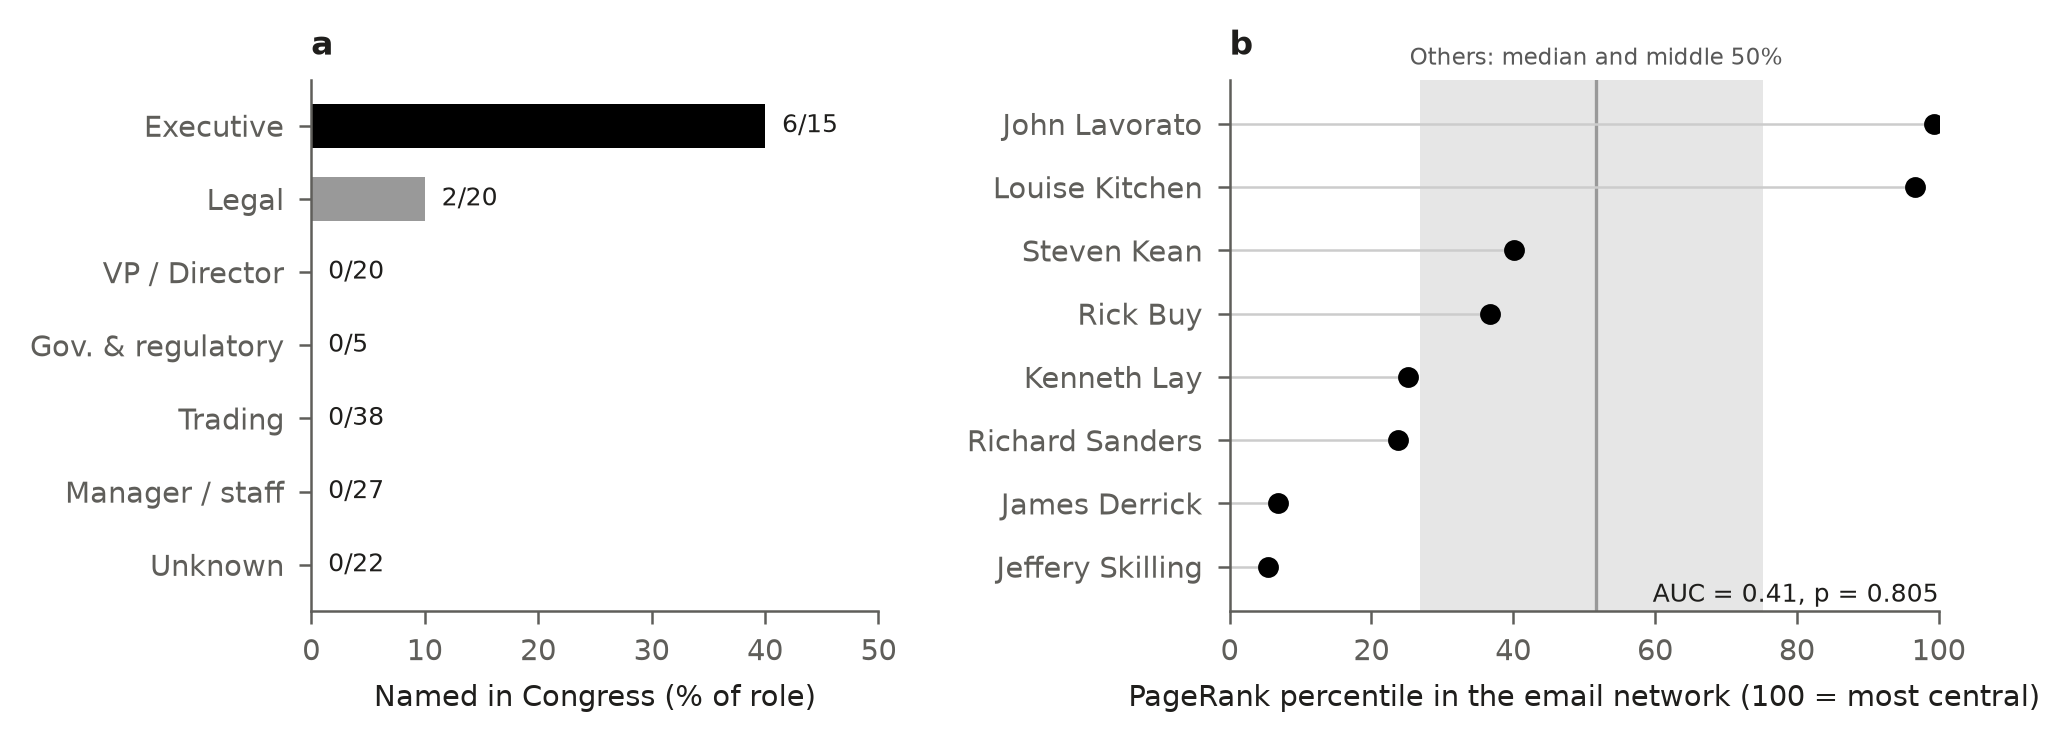
\includegraphics[width=\linewidth]{figures/fig_visibility.png}
\caption{\textbf{Congress named executives, not the center of the email network.}
Network centrality (PageRank percentile) of the 147 connected employees by role, with the 8
employees named in the congressional documents highlighted, and the share of each role that
was named. Named employees are no more central than the others (AUC = 0.41, one-sided
$p = 0.81$, 5,000 label shuffles); six of the eight are executives (Fisher $p < 10^{-5}$).
13 of the 14 network brokers were never named.}
\label{fig:visibility}
\end{figure}

\subsection*{Congress's subjects barely appear in the employees' emails}
The next step of our story is to find out what Congress investigated. We split the ten
documents into 2,438 passages of about 180 words and fitted an LDA topic model
\cite{blei2003}. We named the topics, not the passages, by hand from their most frequent
words and strongest passages, and checked the names on 30 passages: 26 fit the name of their
main topic. A second model (NMF \cite{lee1999}) finds a matching topic for each, although
passage assignments vary between LDA runs (mean NMI 0.39 across seeds), so we use the topics
only to define what Congress investigated, not to classify texts.

We merged the topics into eight themes, wrote a term list for each, and applied these term
lists to the employees' emails. We kept only emails written by a person, without forwarded
text, duplicates or pasted news articles. The tagging is precise: in a hand check, 27 of 30
tagged emails were about their theme (precision 0.90, 95\% CI 0.74--0.97 \cite{wilson1927}),
and only 1 of 30 untagged emails was about a theme.

Congress's subjects barely appear in the emails (Fig.~\ref{fig:coverage}). In the hearings
and reports, the largest themes are Arthur Andersen and its audits (33\% of passages), the
special purpose entities and Raptor hedges (23\%) and the LJM partnerships (22\%), followed
by the bankruptcy and its impact on employees (13\%); energy trading appears in only 10\%. In
the employees' emails, by contrast, only \chk{0.5\%} touch any of the seven finance themes.
% Per word of text,
% Congress used the terms of the Andersen theme 93 times more often than the employees and the special-purpose-entity terms 73 times more often.

Energy, however, is the theme that appears most often in the employees' emails, in \chk{13\%}
of them. To identify what the central people wrote about instead, we fitted an NMF topic model
with 10 topics to the emails, without the congressional themes. The central core's emails are
about contracts, legal paperwork and master agreements, as well as energy markets. None of the
ten email topics concerns the subjects of the congressional investigation. Even the executives
Congress named wrote mostly about California energy-market regulation (\chk{21\%}) and
meetings (\chk{18\%}).

\begin{figure}[t]
\centering
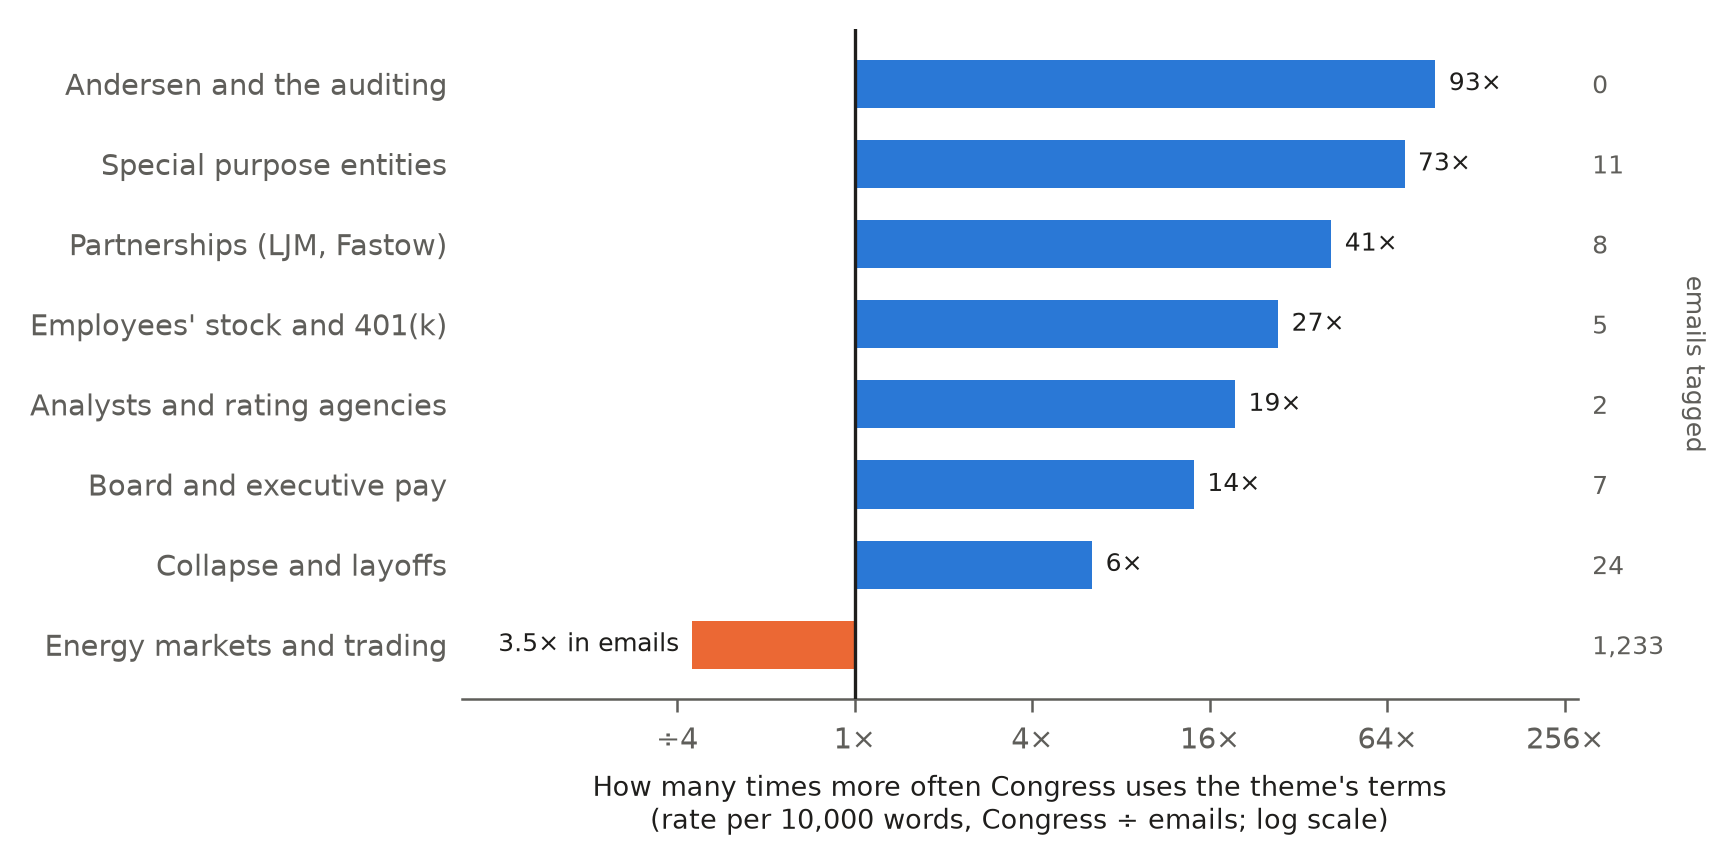
\includegraphics[width=\linewidth]{figures/fig_theme_coverage.png}
\caption{\textbf{Congress and the employees used different vocabularies.} For each theme,
how many times more often the congressional documents use its terms than the employees'
own email text (terms per 10,000 words; log scale). Energy trading is the only theme the
emails use more often. Numbers give the emails tagged with each theme. Theme tagging was
checked by hand (precision 0.90, 95\% CI 0.74--0.97, $n = 30$).}
\label{fig:coverage}
\end{figure}

\subsection*{The central core wrote fewer Congress-theme emails than chance}
If the central employees were part of the activities Congress investigated, they would be
expected to write and receive at least their share of the emails on those subjects. We
tested this by shuffling the theme flags over all own-word emails 10,000 times; each email
keeps its sender and recipients, so people who write a lot are expected to write more theme
emails (\textit{Methods}). The test measures whether a group wrote more or fewer theme
emails than its volume predicts; it says nothing about why.

The central core wrote \chk{8} Congress-theme emails where \chk{25.6} were expected (95\% of
shuffles between \chk{19} and \chk{32}; ratio \chk{0.31}, $p < 0.001$) and received
\chk{12.5} against \chk{23.0} (Fig.~\ref{fig:people}). The named executives did the
opposite: they wrote \chk{7} against \chk{2.3} ($p = 0.007$) and received \chk{8.7} against
\chk{3.5} ($p = 0.004$). The remaining employees wrote \chk{28} against \chk{15.3}. The
deficit is specific to Congress's subjects: the central core wrote energy emails at the
rate its volume predicts (\chk{731} against \chk{700}), and the brokers wrote nearly three
times their share. The result holds when forwarded text is counted, when central is defined
by number of contacts for writing, when receiving is not weighted by the number of
recipients, and when only people named at least ten times count as named; the one exception
is receiving with centrality defined by contacts (\chk{15.8} against \chk{13.0}). Most
Congress-theme emails were written late: \chk{25} of the \chk{45} in November 2001, the month
Enron restated its earnings and lost its investment-grade credit rating, days before its
bankruptcy on 2 December.

\begin{figure}[t]
\centering
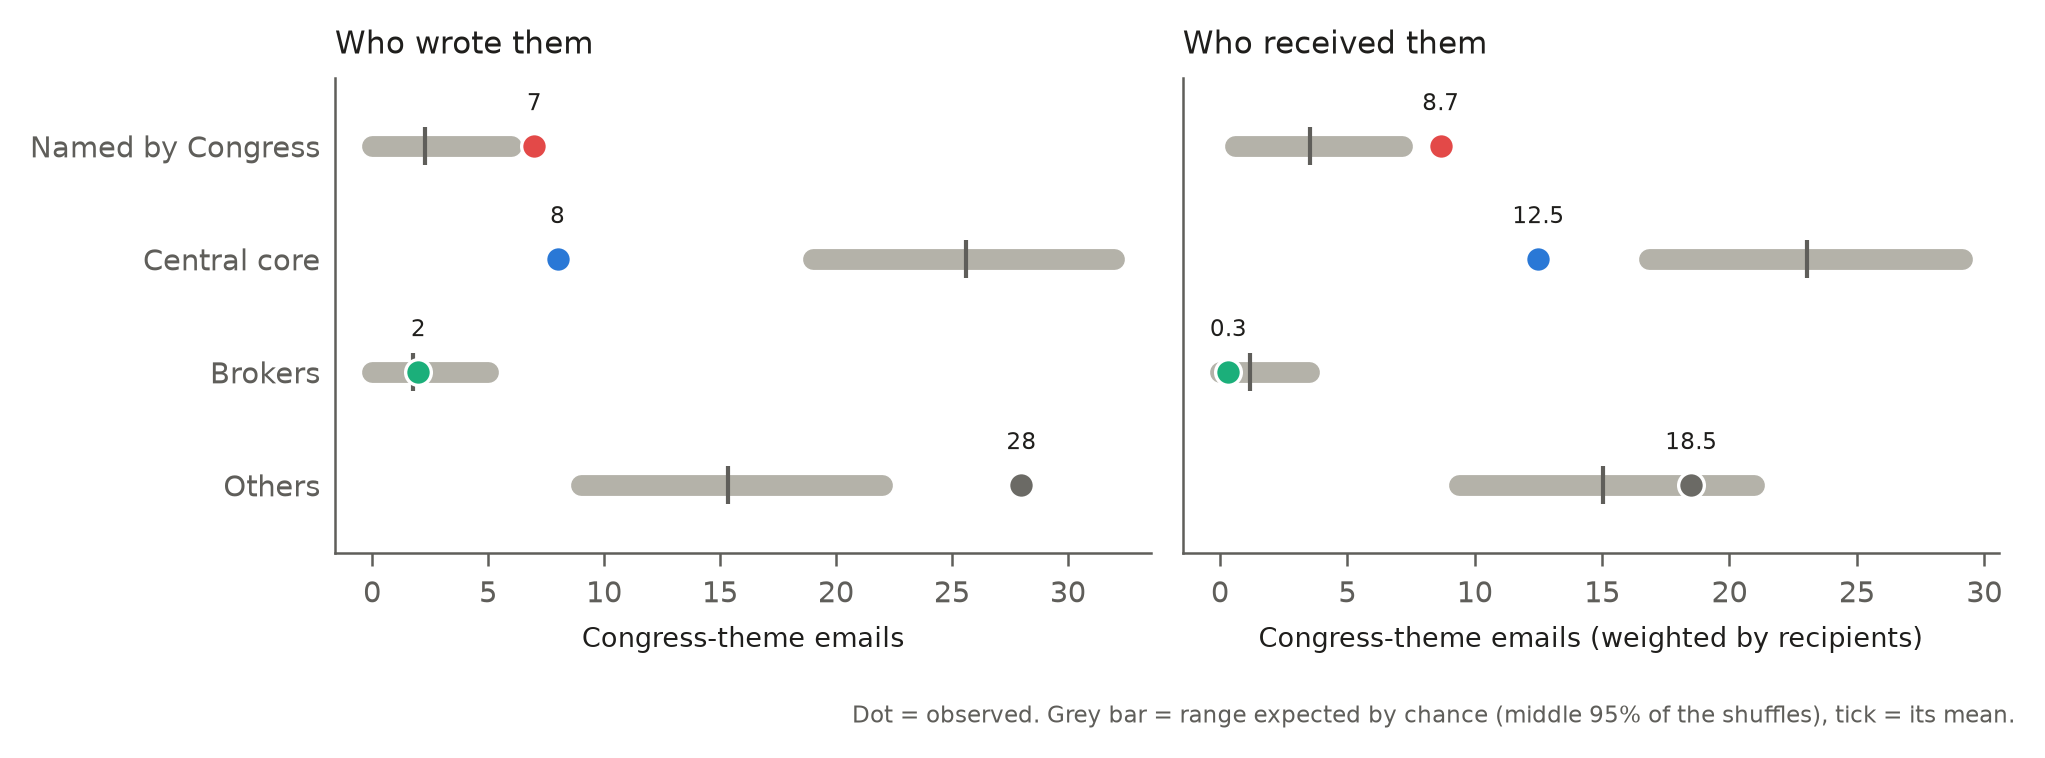
\includegraphics[width=\linewidth]{figures/fig_email_people.png}
\caption{\textbf{The central core wrote and received fewer Congress-theme emails than
chance predicts; the named executives more.} Congress-theme emails written (left) and
received (right; each email weighted by one over its number of recipients) by each group,
against 10,000 shuffles of the theme flags that keep every person's email volume (bars:
95\% of shuffles; dots: observed). Central core: top 20\% by PageRank; brokers: betweenness
$z \ge 2$ against degree-preserving shuffles.}
\label{fig:people}
\end{figure}

% ---------------------------------------------------------------------
\section*{Discussion}
The congressional investigation and the email network describe two different companies.
The investigation looked at executives and at finance: partnerships, special purpose
entities, the audit and the board. The center of the email network was made up of traders,
lawyers and regulatory staff who wrote about California regulation, gas and power deals and
contracts. The few emails on Congress's subjects were written by the executives Congress
named and by employees at the edge of the network, most of them as the company collapsed.

The result does not mean that the central employees did not know what was happening, nor
that they were uninvolved: we measure what people wrote in their own words, in the emails
that survive, not what they knew or did. It also does not mean that Congress looked in the
wrong place. The subjects it investigated lived in a part of the company that the corpus
barely shows.

That is the main limitation, and one we found ourselves. FERC collected the mailboxes of the
energy-trading business it was investigating; the finance employees at the heart of the
congressional account (Andrew Fastow, Richard Causey, Ben Glisan, Michael Kopper) have no
mailbox in it. In the \chk{76} emails of seven such employees that are visible because they
wrote to the 148, \chk{12\%} are on Congress's themes, more than twenty times the rate of
the 148. Part of the gap between the two views is therefore built into which records were
preserved, and an analysis of any surviving archive should ask the same question. Further
limits are that one person did the hand labeling, the hand-check samples per theme are small,
and the themes are defined by vocabulary; an email can discuss a partnership without naming
it.

With more time we would add a second annotator, extend the analysis to the full corpus and
to the mailboxes released later, and follow how the network's center shifted in the final
months, when the Congress-theme emails appear.

% ---------------------------------------------------------------------
\section*{Materials and Methods}

\subsection*{Email data}
We used the 148 employees of the Enron corpus with their own mailbox \cite{klimt2004},
with full names, departments and roles from public custodian lists, checked by hand. The
database holds the \chk{14,797} emails exchanged among them, plus \chk{185} emails between
the 148 and seven finance and legal employees without a mailbox (Fastow, Causey, Glisan,
Kopper, McMahon, Watkins, Mintz), which we used only for the comparison in the Discussion.
The network is directed and weighted: a tie from $i$ to $j$ counts the emails $i$ sent to
$j$; emails to oneself (1,314) are left out.

For the text analyses we kept emails classified as written by a person (those marked
uncertain with a probability of at least 0.8 included), removed Outlook synchronization
logs, and kept each sender's own words: text before the first forwarded or quoted message,
without lines quoted with ``>''. Forwarding headers were removed line by line up to the
first line of real text, because removing a fixed number of lines deleted about 230
lines of the senders' own text in 218 emails. Lines that occur in at least 15 emails
(signatures, disclaimers) and duplicates of the same text by the same sender were removed,
and long emails ($\ge$150 words) with signs of a pasted news article (bylines, news
agencies, newspaper names) were set aside. This leaves \chk{9,498} emails
(14,982 $\to$ 13,475 human-written $\to$ 9,922 with at least five words of own text
$\to$ 9,620 unique $\to$ \chk{9,498} without pasted articles).

\subsection*{Congressional documents}
We downloaded the full text of the eight congressional hearings on Enron held between
December 2001 and February 2002 and of two Senate staff reports from July and October 2002
\cite{senate2002board,senate2002oversight,congress2002hearings} from govinfo.gov. Of 14,573
paragraphs we kept 11,421, removing headings, footnotes, procedural lines and the speaker
labels that open each turn, and joined consecutive paragraphs into 2,438 passages of about
180 words (median 210) that keep questions and answers together. Words were lemmatized with
spaCy \cite{spacy}; we removed stopwords, words of hearing procedure and the surnames of
speakers, except those of the people under investigation (195,512 content words, 8,762
distinct; the rank--frequency distribution follows Zipf's law with slope $-1.03$). People
named in the documents were found with spaCy's named-entity recognizer (298 people named at
least three times, 6 of them among the 148) and, for the analyses, from a hand-checked list
of mentions of the 148 (8 people).

\subsection*{Network measures}
Reciprocity (the share of directed ties that are returned) was measured on the directed
network; clustering (the share of a person's pairs of contacts who are themselves linked),
transitivity and path length on the undirected network without weights (path lengths within
the largest connected part, 147 people). Each statistic was compared with 1,000
degree-preserving shuffles \cite{maslov2002}: repeatedly, two links A--B and C--D are swapped
to A--D and C--B (for reciprocity, directed swaps that keep each person's numbers of senders
and recipients), so that every person keeps the same number of contacts while who is linked
to whom becomes random. This null model tests whether a pattern goes beyond what the number
of contacts alone produces. Statistics were also compared with 1,000 random graphs with the
same number of people and links, and $z$-scores are $(x - \bar{x}_{\mathrm{null}}) /
s_{\mathrm{null}}$, the distance from the null mean in standard deviations. The rich-club
coefficient, the share of possible links present among the people with more than $k$
contacts, was divided by its mean in the shuffles \cite{colizza2006}, so that values above 1
mean the best-connected people are linked more than their number of contacts implies; the
links among the 15 executives were also compared with 5,000 random sets of 15 employees.
Mixing by role and department was measured by Newman's assortativity coefficient $r$
\cite{newman2003}, computed from the email between groups (weighted by email volume and,
separately, by links only) and compared with 5,000 shuffles of the labels.

\subsection*{Centrality and the congressional record}
An employee counts as named if the ten congressional documents of the text analysis mention
them at least once. Mentions were found by matching the forms of each employee's name in the
documents (for example ``Mr.~Skilling'', ``Rick Buy'', ``Richard Buy''); matches to a different
person were removed, and 140 of the 828 mentions, at least one per named employee, were
checked by hand against the surrounding text, with AI assistance (8 employees named). Centrality was measured in five
ways: PageRank \cite{brin1998} on the directed network weighted by emails (who receives email
from well-connected people), emails received, emails sent, and, on the undirected network,
betweenness \cite{freeman1977} (who lies on short paths; distance = 1/emails) and eigenvector
centrality (who is linked to well-linked people). For each measure, the area under the ROC curve (AUC) is the probability that a randomly
chosen named employee ranks above a randomly chosen unnamed one (0.5: no difference; below
0.5: named employees rank lower). Because only
8 employees are named, the AUC was compared with 5,000 shuffles of the named label among the
147 connected employees (one-sided $p$: the share of shuffles with an AUC at least as high).
Most employees have a betweenness of zero, so its AUC mainly reflects ties, which is why
brokers are defined by betweenness $z$-scores instead (below). Executives' share among the named was tested with Fisher's exact test. Centrality describes
communication among the 148, not the whole company: PageRank agrees only moderately with the
full corpus (Spearman $\rho = 0.40$). PageRank misses
influence that does not travel by email, and mentions reflect what the investigation asked
about, not who mattered inside the company.

\subsection*{Brokers}
Betweenness centrality \cite{freeman1977} was computed with distance = 1/emails, so that
frequent contact makes a short path, and expressed as a $z$-score against 100
degree-preserving shuffles; brokers have $z \ge 2$ and at least five contacts. The $z$-score
removes the bridging that a person's number of contacts alone would produce; betweenness
captures position on short paths, not whether information actually passed through a person.
How widely a person's email is spread over the communities was measured by the participation
coefficient $P_i = 1 - \sum_c (k_{ic}/k_i)^2$ \cite{guimera2005}, where $k_{ic}$ is the email
$i$ exchanges with community $c$ and $k_i$ all of $i$'s email ($P = 0$ when all of it stays in
one community). Named and other employees were compared with Mann--Whitney tests and, to
control for seniority, by shuffling the named label only within role groups. Central
employees are the top 20\% by PageRank (30 people); crossed with being named, they define
the public faces (central and named), the hidden core (central, not named) and the named but
peripheral (named, not central).

\subsection*{Communities}
Communities were found on the undirected network in which each link is weighted by the
number of emails exchanged in both directions (self-emails removed; one employee without
links left out; 147 people, 1,444 links). We ran the Louvain algorithm \cite{blondel2008}
(resolution 1) with 50 random seeds and kept the partition with the highest modularity $Q$
\cite{newman2004}: the share of email inside communities minus the share expected if everyone
emailed in proportion to their total volume. Because Louvain finds modular partitions even in random networks, we compared $Q$ with 100
degree-preserving shuffles \cite{maslov2002}, measured stability across runs, and compared the
communities with departments and roles by NMI \cite{danon2005} against 1,000 label shuffles.

\subsection*{Topics, themes and tagging}
LDA \cite{blei2003} and NMF \cite{lee1999} were fitted to the passages with 10 topics; we
compared between 6 and 15 topics, stability across seeds varied little, and we kept 10 for
interpretability. The topics were named by hand from their top words and strongest passages
and checked on 30 passages. The eight themes were formed by merging the LDA topics on special
purpose entities and the Raptor hedges, and those on Andersen and accounting rules. We did not
tag emails with the topic model itself, because its topics describe the vocabulary of the
hearings, it assigns every text to some topic, and its assignments shift between runs.
Instead, each theme has \emph{name} terms, specific words that belong only to the subject
(e.g., LJM, Chewco, Raptor, Andersen); \emph{general} terms, which also occur in everyday
business language (e.g., partnership, audit, bonus); and, for the seven finance themes,
\emph{exclude} terms of the California energy crisis and of ISDA agreements. A text has a
theme if it contains one name term, or two different general terms and no exclude term.
Exclude terms prevent texts on the California energy crisis from being wrongly tagged: they
stop the finance themes from being triggered by their general words, while a name term still
counts. The same rule tags the Congress passages and the employees' emails. Coverage is the
share of texts with a theme and, independent of text length, the theme's term matches per
10,000 words. A Congress-theme email is one tagged with any of the seven finance themes. The
eighth theme, energy trading, also comes from the congressional topics but is the employees'
everyday business, so energy emails serve as a contrast.

We checked the term lists by hand on 89 emails, shown in random order without saying which
method had tagged them: emails tagged by the term lists, emails tagged only by an earlier
similarity method (TF-IDF), and 30 untagged emails. Six emails no longer tagged by the final
lists were left out, and intervals are Wilson intervals \cite{wilson1927}; the TF-IDF method
proved mostly off-topic (precision 0.39, $n = 23$). As a supplementary method, each email of
at least 30 words was split into chunks of about 180 words, embedded with a sentence
transformer (all-mpnet-base-v2) \cite{reimers2019}, and compared with the mean embedding of
each theme's passages. An email was tagged if it was among the 1\% of emails most similar to
the theme, the theme was the one it was most similar to, and it contained no exclude term;
the threshold is set among the emails because hearings and emails are written so differently
that even off-topic passages are more similar to a theme than almost any email. These tags
serve only as a check: energy, the emails' main subject, works as a positive control (13 of
its 23 tags also carry the energy term list). Its new tags were not checked by hand; among the
86 emails already labeled, it repeats none of the TF-IDF method's 12 errors, and its three
overlaps with the term lists were all judged correct.

\subsection*{Email topics}
To see what the emails are about without the congressional themes, NMF was fitted to TF-IDF
weights of the \chk{6,209} emails with at least 20 words of their own text (10 topics). The
topics were named by hand from their top words and strongest emails; each email was assigned to
its strongest topic (or none, below a weight of 0.02), and topic shares were computed for each
group of senders (\textit{Permutation test}).

\subsection*{Permutation test}
Each employee belongs to one group, assigned in this order: named by Congress (8); central
core, the top 20\% by PageRank (28); brokers, betweenness $z \ge 2$ in both the weighted and
the unweighted network and at least five contacts (7); and the others (105). For each group
we counted the Congress-theme emails (term-list tags, any of themes 1--7) its members wrote
and received;
an email with $n$ recipients other than the sender counts $1/n$ for each. The theme flags
were shuffled over all own-word emails 10,000 times, which keeps every sender's and
recipient's email volume and the number of theme emails, and we report the observed count,
the expected count, the central 95\% of shuffles and one-sided $p$-values.

\subsection*{Data and code}
Code, term lists, hand labels and the results tables are available at
\url{https://github.com/andrejanisic/enron-socialgraphs} [TODO: make public or adjust].
Analyses used Python 3.14, NetworkX \cite{hagberg2008}, scikit-learn \cite{pedregosa2011},
spaCy \cite{spacy} and sentence-transformers \cite{reimers2019}.

\acknow{We thank the instructors and teaching assistants of DTU course 02805 Social Graphs
and Interactions.}
\showacknow{}

\bibliography{references}

\end{document}
